\documentclass{article}

\usepackage{../packages/definitions}

\title{Molecular Dynamics Simulations: Final Report}
\author{Adrià Meca Montserrat}
\date{\today}

\begin{document}
  \maketitle

  \section{Molecular Dynamics Simulations code}

  \subsection{Introduction}

  We consider an isolated system of \(N=125\) particles with density \(\rho=0.7m/\sigma^{3}\) trapped in a region with PBC. Initially, the particles are located at the vertices of a simple cubic lattice with a bimodal velocity distribution, with which the kinetic energy~\(K\) is compatible with \(k_{B}T=100\epsilon\). Then, we let the system evolve through the action of an integrator ({\em Velocity Verlet} or \emph{Euler}) for \(10^{4}\) time steps, and we analyze its thermodynamic properties.

  The Lennard-Jones potential describes the interactions between particles:
  \[
    u_{LJ}(r)=4\biggl[\Bigl(\frac{1}{r}\Bigr)^{12}-\Bigl(\frac{1}{r}\Bigr)^{6}\biggr].
  \]
  Here, it is written in reduced units since it is more natural to do simulations with dimensionless quantities. We introduce a \emph{cutoff} parameter \(\coff=L/4\) that establishes a distance above which interactions are ignored. This reduces the computational cost, but produces discontinuities in the potential that we must fix with truncation:
  \[
    u_{LJ}(r)=%
    \begin{cases}
      u_{LJ}(r)-u_{LJ}(\coff)&r\le \coff,\\0&r>\coff.
    \end{cases}
  \]

  The Velocity Verlet integrator uses velocities to take the system to the next dynamic step:
  \begin{align*}
    r_{i}(t+\Delta t)&=r_{i}(t)+v_{i}(t)\Delta t+\frac{f_{i}(t)}{2m_{i}}{\Delta t}^{2},\\
    v_{i}(t+\Delta t)&=v_{i}(t)+\frac{f_{i}(t)+f_{i}(t+\Delta t)}{2m_{i}}\Delta t.%\label{eq:vel_verlet}
  \end{align*}
  It is a fast and convenient algorithm to use when the system interacts with a thermal bath. On the other hand, the Euler integrator uses both distances and velocities to update the state of the system:
  \begin{align*}
    r_{i}(t+\Delta t)&=r_{i}(t)+v_{i}(t)\Delta t+\frac{f_{i}(t)}{2m_{i}}{\Delta t}^{2}+\mathcal{O}({\Delta t}^{3}),\\
    v_{i}(t+\Delta t)&=v_{i}(t)+\frac{f_{i}(t)}{m_{i}}\Delta t+\mathcal{O}({\Delta t}^{2}).%\label{eq:euler}
  \end{align*}
  Its disadvantages are the energy drift and the lack of symmetry under time reversal. In both equations, \(f_{i}\) is the force associated with the Lennard-Jones potential.

  \subsection{Results}

  Figure~\ref{fig:vel_verlet} shows the results obtained with the Velocity Verlet integrator. For \(\pass{3}\), \(K\) and \(U\) fluctuate more intensely. However, in both cases the total energy and momentum are conserved.
  \begin{figure}[htb]
    \centering
    \minipage{.45\linewidth}
        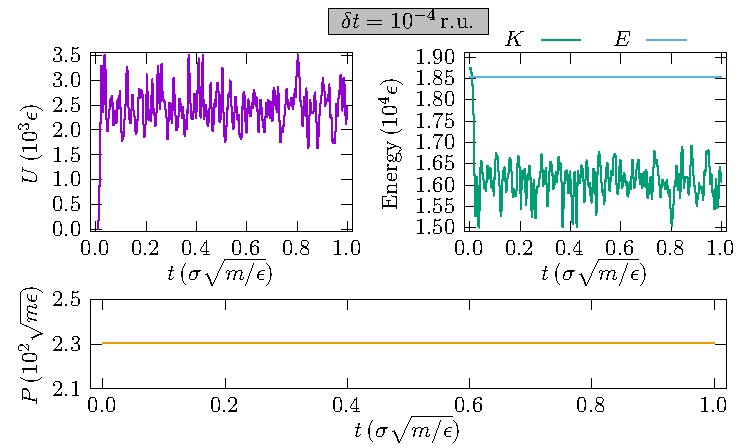
\includegraphics[width=\linewidth]{../figures/vel_verlet_energies_01.pdf}
    \endminipage%
    \minipage{.45\linewidth}
        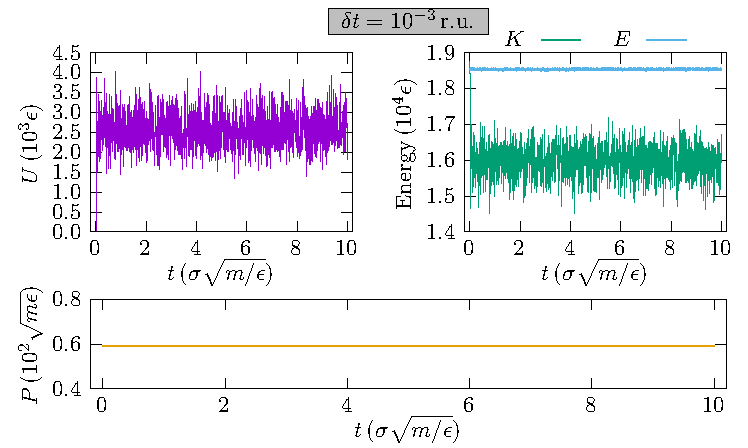
\includegraphics[width=\linewidth]{../figures/vel_verlet_energies_02.pdf}
    \endminipage
    \caption{Energies and total momentum calculated with the Velocity Verlet integrator for different time increments \(\delta t\).}\label{fig:vel_verlet}
  \end{figure}

  On the other hand, Figure~\ref{fig:euler} shows the results obtained with the Euler integrator. For \(\pass{4}\), the energies are reasonable even though the total energy is not preserved. For \(\pass{3}\), however, the energies blow up which is a manifestation of the integrator's flaws. In both cases, the total momentum is a conserved quantity.
  \begin{figure}[htb]
    \centering
    \minipage{.45\linewidth}
        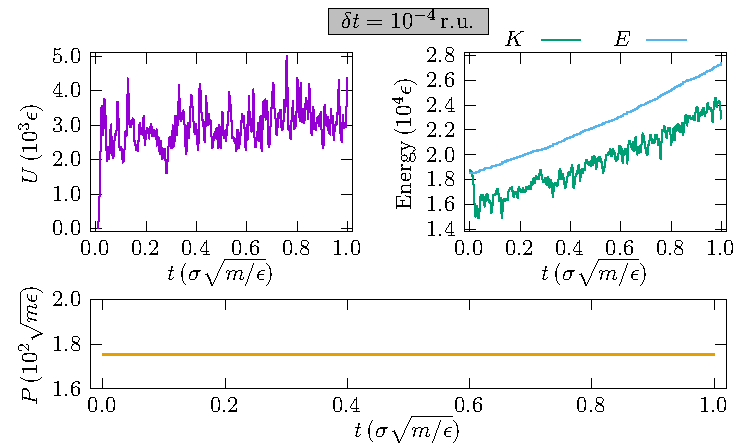
\includegraphics[width=\linewidth]{../figures/euler_energies_01.pdf}
    \endminipage%
    \minipage{.45\linewidth}
        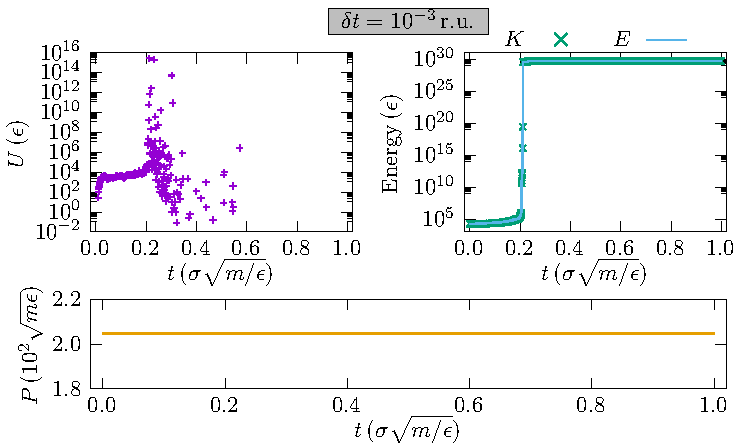
\includegraphics[width=\linewidth]{../figures/euler_energies_02.pdf}
    \endminipage
    \caption{Energies and total momentum calculated with the Euler integrator for different time increments \(\delta t\).}\label{fig:euler}
  \end{figure}

  Finally, Figure~\ref{fig:hist} shows the initial and equilibrium velocity distributions of the particles obtained with the Velocity Verlet integrator for \(\pass{4}\).
  \begin{figure}[htb]
    \centering
    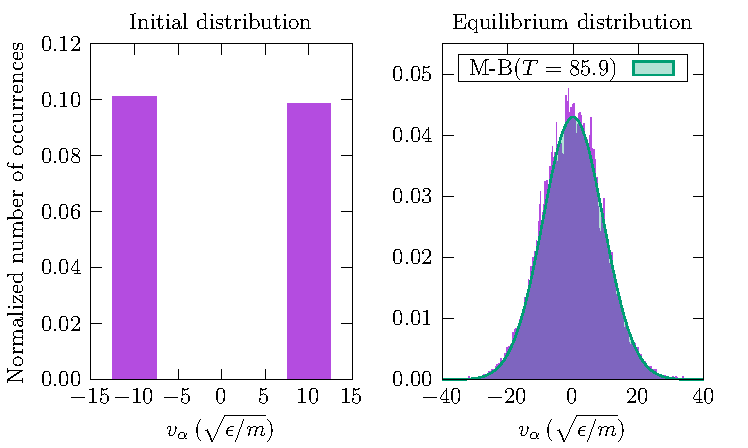
\includegraphics[width=\linewidth]{../figures/vel_verlet_histogram.pdf}
    \caption{Initial and equilibrium velocity distributions of the particles obtained with the Velocity Verlet integrator for \(\pass{4}\).}\label{fig:hist}
  \end{figure}
  The system leaves the initial bimodal distribution as it evolves and cools down, eventually reaching a Maxwell-Boltzmann equilibrium distribution
  \[
    f(v_{\alpha})=\frac{1}{\sqrt{2\pi T}}\exp\Bigl(-\frac{v_{\alpha}^{2}}{2T}\Bigr).
  \]

  \section{Properties of a Lennard-Jones liquid}

  \subsection{Introduction}

  We consider a system of \(N=125\) argon atoms trapped in a region with PBC. Initially, the atoms are at rest at the vertices of a simple cubic lattice. After melting the crystalline structure, we put the system in contact with a thermal bath at \(k_{B}T=2\epsilon\) using an Andersen thermostat, and let it evolve with the Velocity Verlet integrator for \(10^{6}\) time steps. The objective is to obtain the thermodynamic properties of the system.

  As in the previous section, the atoms interact through the Lennard-Jones potential and the simulation is carried out with reduced units. Once finished, we retrive the physical units multiplying the different quantities by an appropriate combination of parameters (Table~\ref{tab:units}).

  \subsection{Results}

  Figure~\ref{fig:liquid} shows the energies and pressure of the system for several density values. As density increases, the space available for the atoms shrinks, they collide more frequently and pressure raises.
  \begin{figure}[htb]
    \centering
    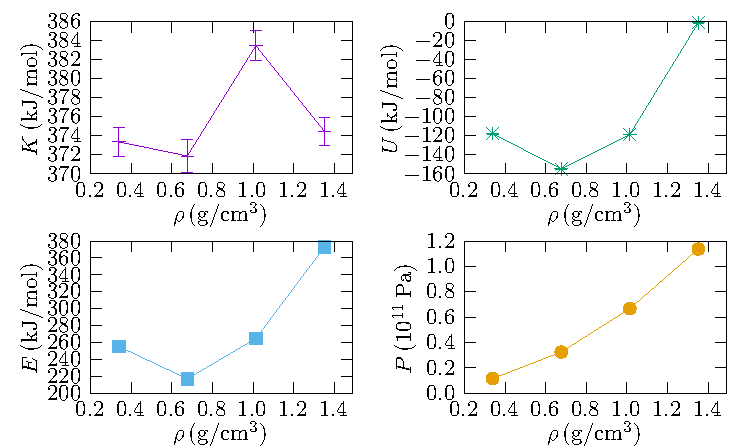
\includegraphics[width=\linewidth]{../figures/liquid_quantities.pdf}
    \caption{Equilibrium values of the averages of the energies and pressure of the system evaluated with the Velocity Verlet integrator. The error bars come from the block average method.}\label{fig:liquid}
  \end{figure}

  We also study the time evolution of the Mean Square Displacement (MSD) of argon atoms for \(\rho=0.6m/\sigma^{3}\) and \(k_{B}T=2\epsilon\) without PBC; see Figure~\ref{fig:msd}. We repeat the simulation \(10\) times and we average over the realizations to obtain a more accurate result. Since
  \[
    \text{MSD}(t)=6Dt\qquad(t\to\infty),
  \]
  we can calculate the diffusion coefficient~\(D\) with a linear regression:
  \[
    D=\frac{a}{6}=9.9743\pm0.0008\,\textup{\AA}^{2}\!/\mathrm{ps},
  \]
  where \(a\) is the slope of the regression line.
  \begin{figure}[htb]
    \centering
    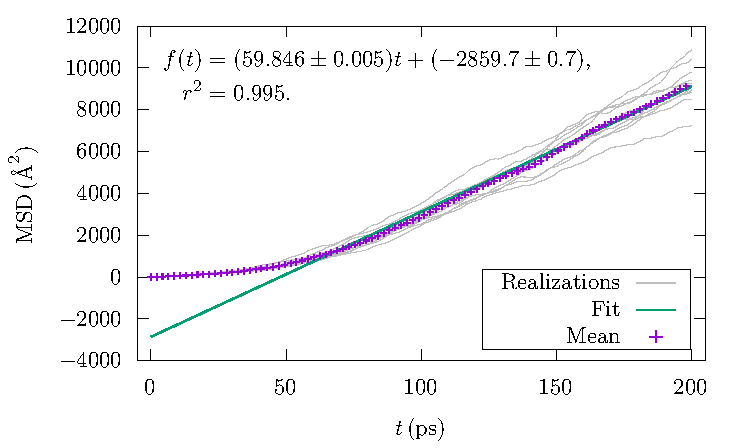
\includegraphics[width=\linewidth]{../figures/msd.pdf}
    \caption{Mean Square Displacement as a function of time for a system of \(125\) argon atoms with \(\rho=0.6m/\sigma^{3}\) and \(k_{B}T=2\epsilon\) without PBC.}\label{fig:msd}
  \end{figure}

  \begin{table}[htb]
    \centering
    \caption{Combinations of parameters required to retrieve the physical units of different quantities of interest.}\label{tab:units}
    \begin{tabular}{ll}\hline
      Physical quantity & Unit                         \\\hline\hline
      Leght             & \(\sigma\)                   \\
      Energy            & \(\epsilon\)                 \\
      Mass              & \(m\)                        \\
      Time              & \(\sigma(m/\epsilon)^{1/2}\) \\
      Velocity          & \((\epsilon/m)^{1/2}\)       \\
      Force             & \(\epsilon/\sigma\)          \\
      Pressure          & \(\epsilon/\sigma^{3}\)      \\
      Temperature       & \(\epsilon/k_{B}\)           \\\hline
    \end{tabular}
  \end{table}

  \begin{thebibliography}{99}
    \bibitem{Calero} C. Calero, {\em Slides on Molecular Dynamics Simulations}, UB-UPC, 2021.
    \bibitem{DrMeca} I have created a \href{https://github.com/AdriaMeca/Molecular-Dynamics-Simulations.git}{GitHub repository} that contains the codes I have used to obtain the results.
  \end{thebibliography}

\end{document}
